\documentclass{standalone}
\usepackage{tikz}
\usetikzlibrary{patterns, positioning}


\begin{document}
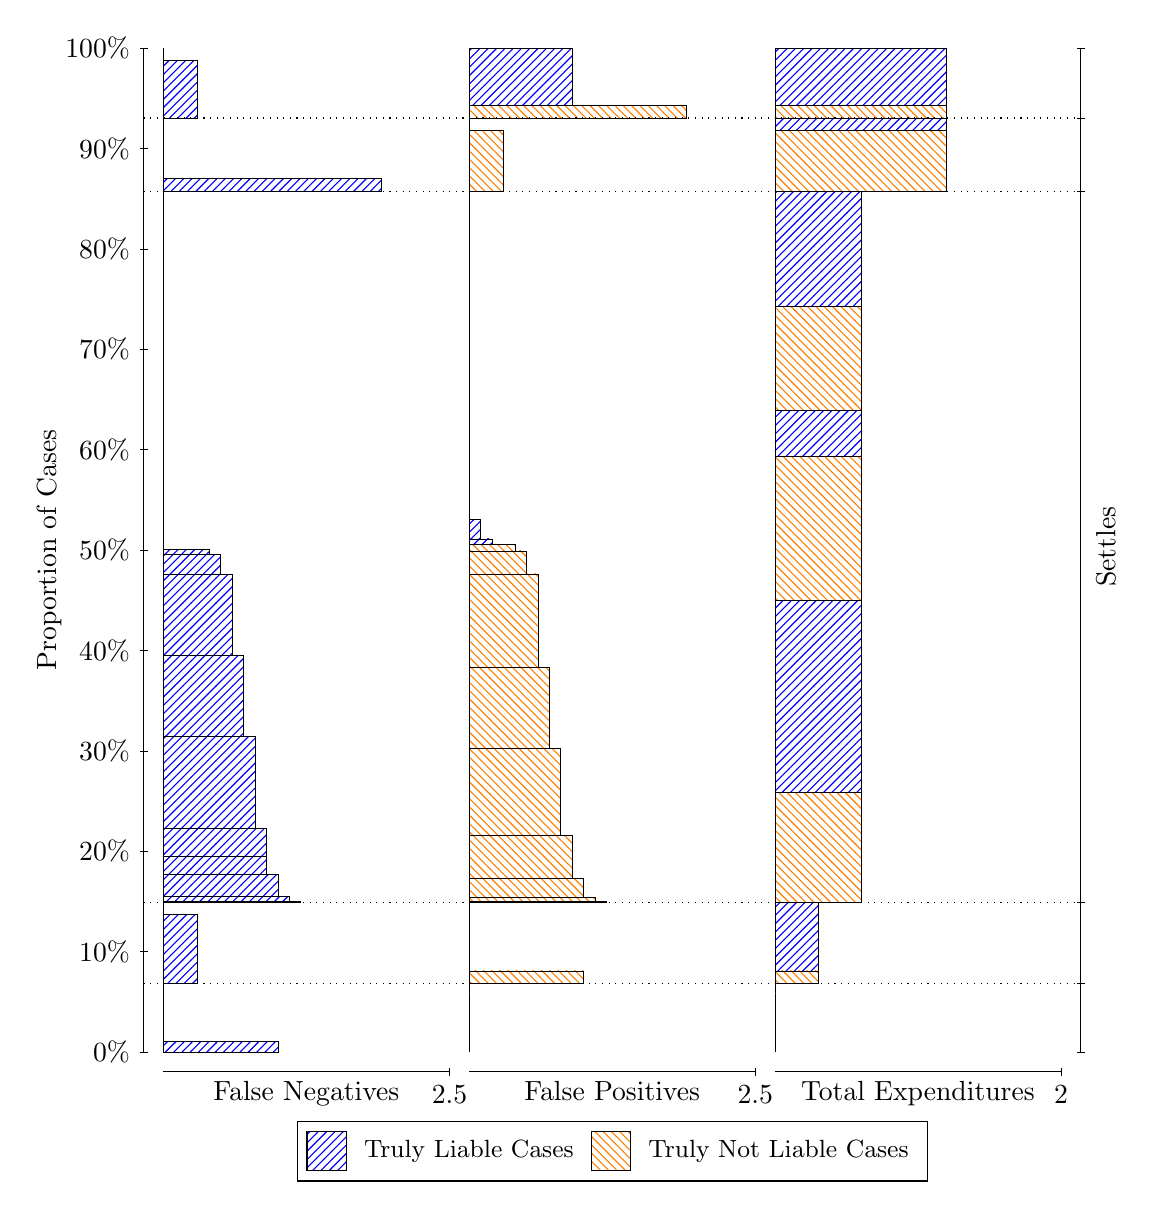
\begin{tikzpicture}
\draw[black, very thin] (1.5,1.75) -- (1.5,14.5);
\node[rotate=90, text=black, anchor=center] at (0.3, 8.125) {Proportion of Cases};
\draw[black, very thin] (1.45,1.75) -- (1.55,1.75);
\node[text=black, anchor=east] at (1.45, 1.75) {0\%};
\draw[black, very thin] (1.45,3.025) -- (1.55,3.025);
\node[text=black, anchor=east] at (1.45, 3.025) {10\%};
\draw[black, very thin] (1.45,4.3) -- (1.55,4.3);
\node[text=black, anchor=east] at (1.45, 4.3) {20\%};
\draw[black, very thin] (1.45,5.575) -- (1.55,5.575);
\node[text=black, anchor=east] at (1.45, 5.575) {30\%};
\draw[black, very thin] (1.45,6.85) -- (1.55,6.85);
\node[text=black, anchor=east] at (1.45, 6.85) {40\%};
\draw[black, very thin] (1.45,8.125) -- (1.55,8.125);
\node[text=black, anchor=east] at (1.45, 8.125) {50\%};
\draw[black, very thin] (1.45,9.4) -- (1.55,9.4);
\node[text=black, anchor=east] at (1.45, 9.4) {60\%};
\draw[black, very thin] (1.45,10.675) -- (1.55,10.675);
\node[text=black, anchor=east] at (1.45, 10.675) {70\%};
\draw[black, very thin] (1.45,11.95) -- (1.55,11.95);
\node[text=black, anchor=east] at (1.45, 11.95) {80\%};
\draw[black, very thin] (1.45,13.225) -- (1.55,13.225);
\node[text=black, anchor=east] at (1.45, 13.225) {90\%};
\draw[black, very thin] (1.45,14.5) -- (1.55,14.5);
\node[text=black, anchor=east] at (1.45, 14.5) {100\%};

\draw[black, very thin] (13.4,1.75) -- (13.4,14.5);
\draw[black, very thin] (13.35,1.75) -- (13.45,1.75);
\node[anchor=west] at (13.35, 1.75) {};
\draw[black, very thin] (13.35,2.625) -- (13.45,2.625);
\node[anchor=west] at (13.35, 2.625) {};
\draw[black, very thin] (13.35,3.6499) -- (13.45,3.6499);
\node[anchor=west] at (13.35, 3.6499) {};
\draw[black, very thin] (13.35,12.683) -- (13.45,12.683);
\node[anchor=west] at (13.35, 12.683) {};
\draw[black, very thin] (13.35,13.612) -- (13.45,13.612);
\node[anchor=west] at (13.35, 13.612) {};
\draw[black, very thin] (13.35,14.5) -- (13.45,14.5);
\node[anchor=west] at (13.35, 14.5) {};

\draw[black, very thin, pattern color=blue, pattern=north east lines] (1.75,1.75) rectangle (3.2033,1.884);
\draw[black, very thin, pattern color=orange, pattern=north west lines] (1.75,1.884) rectangle (1.75,2.625);
\draw[black, very thin, pattern color=blue, pattern=north east lines] (1.75,2.625) rectangle (2.186,3.4938);
\draw[black, very thin, pattern color=orange, pattern=north west lines] (1.75,3.4938) rectangle (1.75,3.6499);
\draw[black, very thin, pattern color=blue, pattern=north east lines] (1.75,3.6499) rectangle (3.494,3.6659);
\draw[black, very thin, pattern color=blue, pattern=north east lines] (1.75,3.6659) rectangle (3.3487,3.7239);
\draw[black, very thin, pattern color=blue, pattern=north east lines] (1.75,3.7239) rectangle (3.2033,4.008);
\draw[black, very thin, pattern color=blue, pattern=north east lines] (1.75,4.008) rectangle (3.058,4.2312);
\draw[black, very thin, pattern color=blue, pattern=north east lines] (1.75,4.2312) rectangle (3.058,4.593);
\draw[black, very thin, pattern color=blue, pattern=north east lines] (1.75,4.593) rectangle (2.9127,5.7559);
\draw[black, very thin, pattern color=blue, pattern=north east lines] (1.75,5.7559) rectangle (2.7673,6.7893);
\draw[black, very thin, pattern color=blue, pattern=north east lines] (1.75,6.7893) rectangle (2.622,7.8163);
\draw[black, very thin, pattern color=blue, pattern=north east lines] (1.75,7.8163) rectangle (2.4767,8.0674);
\draw[black, very thin, pattern color=blue, pattern=north east lines] (1.75,8.0674) rectangle (2.3313,8.1338);
\draw[black, very thin, pattern color=orange, pattern=north west lines] (1.75,8.1338) rectangle (1.75,12.683);
\draw[black, very thin, pattern color=blue, pattern=north east lines] (1.75,12.683) rectangle (4.5113,12.843);
\draw[black, very thin, pattern color=orange, pattern=north west lines] (1.75,12.843) rectangle (1.75,13.612);
\draw[black, very thin, pattern color=blue, pattern=north east lines] (1.75,13.612) rectangle (2.186,14.34);
\draw[black, very thin, pattern color=orange, pattern=north west lines] (1.75,14.34) rectangle (1.75,14.5);
\draw[black, very thin, pattern color=orange, pattern=north west lines] (5.6333,1.75) rectangle (5.6333,2.491);
\draw[black, very thin, pattern color=blue, pattern=north east lines] (5.6333,2.491) rectangle (5.6333,2.625);
\draw[black, very thin, pattern color=orange, pattern=north west lines] (5.6333,2.625) rectangle (7.0867,2.7811);
\draw[black, very thin, pattern color=blue, pattern=north east lines] (5.6333,2.7811) rectangle (5.6333,3.6499);
\draw[black, very thin, pattern color=orange, pattern=north west lines] (5.6333,3.6499) rectangle (7.3773,3.6625);
\draw[black, very thin, pattern color=orange, pattern=north west lines] (5.6333,3.6625) rectangle (7.232,3.7114);
\draw[black, very thin, pattern color=orange, pattern=north west lines] (5.6333,3.7114) rectangle (7.0867,3.9505);
\draw[black, very thin, pattern color=orange, pattern=north west lines] (5.6333,3.9505) rectangle (6.9413,4.4963);
\draw[black, very thin, pattern color=orange, pattern=north west lines] (5.6333,4.4963) rectangle (6.796,5.6065);
\draw[black, very thin, pattern color=orange, pattern=north west lines] (5.6333,5.6065) rectangle (6.6507,6.6342);
\draw[black, very thin, pattern color=orange, pattern=north west lines] (5.6333,6.6342) rectangle (6.5053,7.8225);
\draw[black, very thin, pattern color=orange, pattern=north west lines] (5.6333,7.8225) rectangle (6.36,8.1126);
\draw[black, very thin, pattern color=orange, pattern=north west lines] (5.6333,8.1126) rectangle (6.2147,8.199);
\draw[black, very thin, pattern color=blue, pattern=north east lines] (5.6333,8.199) rectangle (5.924,8.2654);
\draw[black, very thin, pattern color=blue, pattern=north east lines] (5.6333,8.2654) rectangle (5.7787,8.5165);
\draw[black, very thin, pattern color=blue, pattern=north east lines] (5.6333,8.5165) rectangle (5.6333,12.683);
\draw[black, very thin, pattern color=orange, pattern=north west lines] (5.6333,12.683) rectangle (6.0693,13.452);
\draw[black, very thin, pattern color=blue, pattern=north east lines] (5.6333,13.452) rectangle (5.6333,13.612);
\draw[black, very thin, pattern color=orange, pattern=north west lines] (5.6333,13.612) rectangle (8.3947,13.772);
\draw[black, very thin, pattern color=blue, pattern=north east lines] (5.6333,13.772) rectangle (6.9413,14.5);
\draw[black, very thin, pattern color=orange, pattern=north west lines] (9.5167,1.75) rectangle (9.5167,2.491);
\draw[black, very thin, pattern color=blue, pattern=north east lines] (9.5167,2.491) rectangle (9.5167,2.625);
\draw[black, very thin, pattern color=orange, pattern=north west lines] (9.5167,2.625) rectangle (10.062,2.7811);
\draw[black, very thin, pattern color=blue, pattern=north east lines] (9.5167,2.7811) rectangle (10.062,3.6499);
\draw[black, very thin, pattern color=orange, pattern=north west lines] (9.5167,3.6499) rectangle (10.607,5.048);
\draw[black, very thin, pattern color=blue, pattern=north east lines] (9.5167,5.048) rectangle (10.607,7.4891);
\draw[black, very thin, pattern color=orange, pattern=north west lines] (9.5167,7.4891) rectangle (10.607,9.3165);
\draw[black, very thin, pattern color=blue, pattern=north east lines] (9.5167,9.3165) rectangle (10.607,9.8978);
\draw[black, very thin, pattern color=orange, pattern=north west lines] (9.5167,9.8978) rectangle (10.607,11.221);
\draw[black, very thin, pattern color=blue, pattern=north east lines] (9.5167,11.221) rectangle (10.607,12.683);
\draw[black, very thin, pattern color=orange, pattern=north west lines] (9.5167,12.683) rectangle (11.697,13.452);
\draw[black, very thin, pattern color=blue, pattern=north east lines] (9.5167,13.452) rectangle (11.697,13.612);
\draw[black, very thin, pattern color=orange, pattern=north west lines] (9.5167,13.612) rectangle (11.697,13.772);
\draw[black, very thin, pattern color=blue, pattern=north east lines] (9.5167,13.772) rectangle (11.697,14.5);
\draw[black, dotted] (1.5,2.625) -- (13.4,2.625);
\draw[black, dotted] (1.5,3.6499) -- (13.4,3.6499);
\draw[black, dotted] (1.5,12.683) -- (13.4,12.683);
\draw[black, dotted] (1.5,13.612) -- (13.4,13.612);
\draw[black, very thin] (1.75,1.5) -- (5.3833,1.5);
\node[text=black, anchor=north] at (3.5667, 1.5) {False Negatives};
\draw[black, very thin] (5.3833,1.45) -- (5.3833,1.55);
\node[text=black, anchor=north] at (5.3833, 1.45) {2.5};

\draw[black, very thin] (5.6333,1.5) -- (9.2667,1.5);
\node[text=black, anchor=north] at (7.45, 1.5) {False Positives};
\draw[black, very thin] (9.2667,1.45) -- (9.2667,1.55);
\node[text=black, anchor=north] at (9.2667, 1.45) {2.5};

\draw[black, very thin] (9.5167,1.5) -- (13.15,1.5);
\node[text=black, anchor=north] at (11.333, 1.5) {Total Expenditures};
\draw[black, very thin] (13.15,1.45) -- (13.15,1.55);
\node[text=black, anchor=north] at (13.15, 1.45) {2};



\node[text=black, centered, rotate=90] at (13.72, 8.1664) {Settles};



\draw (7.449999999999999,1.5) node[draw=none] (baseCoordinate) {};
\begin{scope}[align=center]
        \matrix[scale=0.5, draw=black, below=0.5cm of baseCoordinate, nodes={draw}, column sep=0.1cm]{
            \node[rectangle, draw, minimum width=0.5cm, minimum height=0.5cm, pattern color=blue, pattern=north east lines] {}; &
            \node[draw=none, font=\small, text=black] (B) {Truly Liable Cases}; &
            \node[rectangle, draw, minimum width=0.5cm, minimum height=0.5cm, pattern color=orange, pattern=north west lines] {}; &
            \node[draw=none, font=\small, text=black] (B) {Truly Not Liable Cases}; \\
            };
\end{scope}

\end{tikzpicture}
\end{document}